\documentclass[a4paper,10pt]{book}
\usepackage[utf8x]{inputenc}
\usepackage{graphicx}
\usepackage{listings}
\usepackage[nodayofweek]{datetime}
\usepackage{color}

\definecolor{lightgrey}{RGB}{230,230,230}

\begin{document}

\title{Dotcount User Guide}
\date{\today}
\author{Joacim Thomassen}

\maketitle


\lstset{ 
literate={²}{{$^2$}}1,
frame=single,
basicstyle=\footnotesize,
backgroundcolor=\color{lightgrey}
}

\chapter{System requirements}
\label{chap:requirements}
Dotcount was built and tested on Ubuntu 10.04 LTS. A workstation with this
system up and running is thus necessary to use Dotcount as it is. If you don't
already have an Ubuntu workstation you're advised to seek information and
guidance from Ubuntu's own website ubuntu.com.

Dotcount depends on another software component, the NetPBM library. Ubuntu will
install this component for you if you search for libnetpbm10 in the Ubuntu
Software Center and select install. 

With Ubuntu and the NetPBM component installed your final step is to install
Dotcount itself. This is done by copying the executable file called dotcount to
your own system. Copy this single file to your system's local program
path\footnote{local program path = /usr/local/bin/}. See listing
\ref{lst:copyinstall} for the command line you must enter in the Terminal
program. That's it. You now have a system with Dotcount installed.

\begin{lstlisting}[caption={Install program with copy command. Replace
MYMEDIA with the name given to your media containing dotcount.},
label=lst:copyinstall]
sudo cp /media/MYMEDIA/bin/dotcount /usr/local/bin/
\end{lstlisting}


\chapter{Overview}
\label{chap:overview}

\begin{figure}[htb]
  \centering
  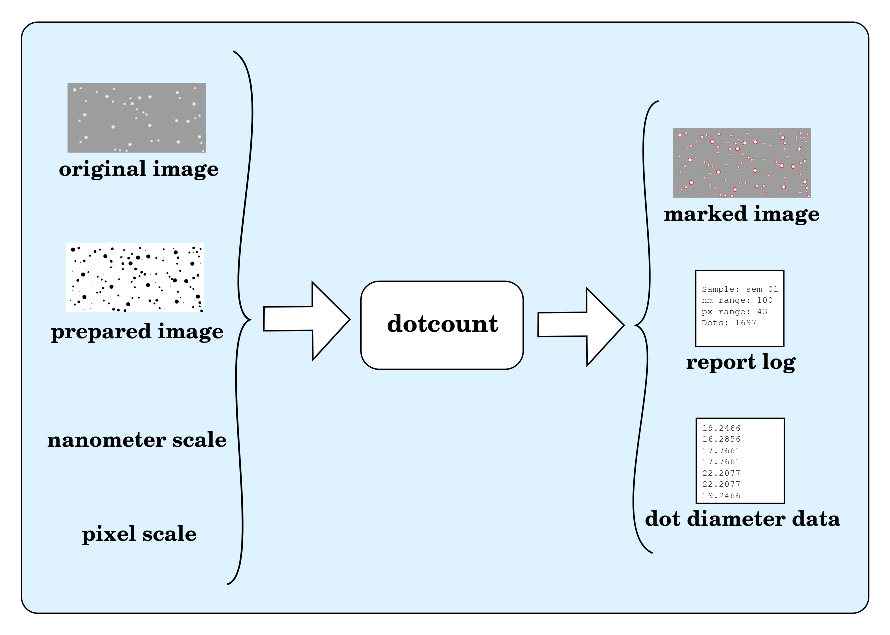
\includegraphics[width=0.8\textwidth]{dotcountoverview}
  \caption{Program overview}
  \label{fig:progoverview}
\end{figure}

Dotcount is an image analysis program to count dots and approximate each dot's 
diameter. Dotcount has a command line interface and expects to be started
together with the original image, a prepared version of the original image, and
two scale sizes. The program then locates all the dots, marks them in a copy
of the original image and reports the total amount and approximated dot
diameter. This report is stored in two text files and can be used in further
statistical analysis of the results. For an overview see figure
\ref{fig:progoverview}.


\chapter{Preparing program input}
\label{chap:preparing}
Dotcount has so far been used to analyze SEM images showing quantum dots in
the layer structure of a new material. The laboratory image must have meta data
about the scale to give meaningful approximations about dot diameters. Dotcount
do need some manual help to reveal and separate out the dots from the
background and image noise. This is done by preparing the lab image for
Dotcount in an standard image editor like The Gimp. 

\begin{figure}[htb]
\centering
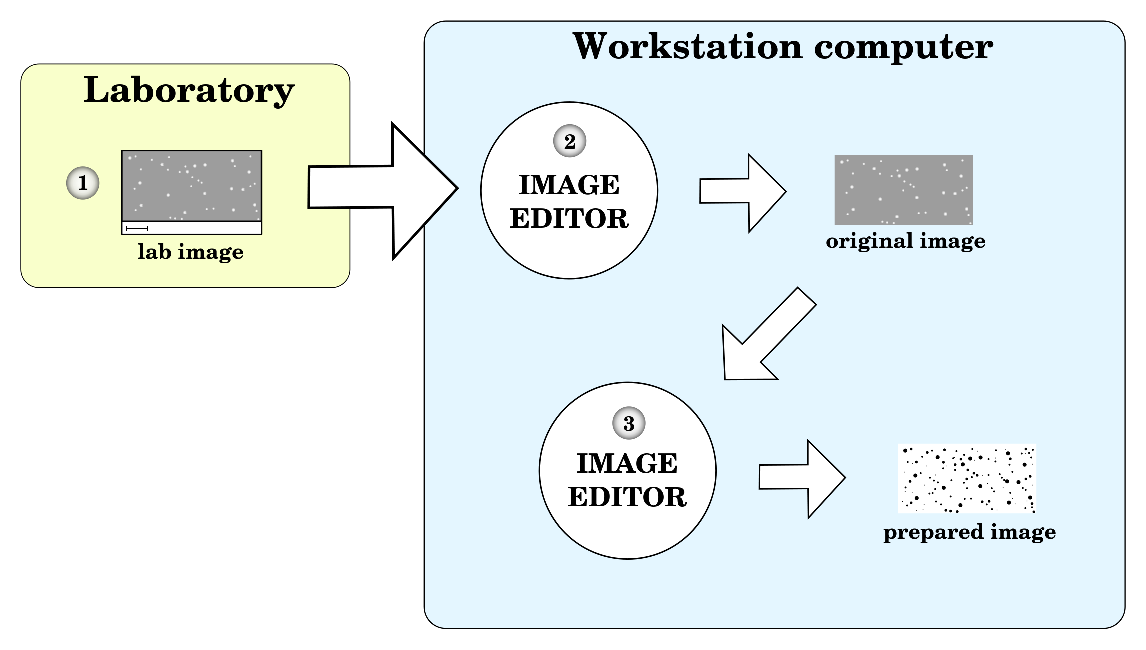
\includegraphics[width=0.8\textwidth]{programinput}
\caption{Program input preparation}
\label{fig:proginput}
\end{figure}

Thresholds and curves are
used to separate tone values in the greyscale image and must result in a binary
image with only white and black values. This preparation is documented in the
instructional video ``Input preparation''.

In figure \ref{fig:proginput} an overview of the preparation procedure is
illustrated. The details of this image editing routine is presented in the
instructional video and are outlined in listing \ref{lst:preproutine}.

\begin{enumerate}
  \label{lst:preproutine}
  \item Image the surface of your sample material. Save the image as a digital
image like TIFF or similar.
  \item Open the lab image in an image editor like The Gimp. Do the following.
  \begin{enumerate}
    \item Extract scale information.
    \item Crop image so only the surface part that you wish to analyze is
visible. No borders or meta data like logo etc. can be present.
    \item Increase contrast if necessary.
    \item Convert the image to PNM by saving it in this format. This saved
image is called the original image.
  \end{enumerate}
  \item Work on the original image (cropped PNM) to be sure you have the
identical image data for the prepared image we're about to make.
  \begin{enumerate}
    \item Adjust levels and curves to get the cleanest dot representation. 
    \item Save the image with a different name, like sample01prepared.pnm. This
saved image is called the prepared image.
  \end{enumerate}
\end{enumerate}

\chapter{Program usage}
\label{chap:usage}
Dotcount is executed from the command line and will save it's output to the
same directory as it is invoked from. If you have your original image and
prepared image in a directory named \textit{sample1} you could invoke dotcount
from this directory and the result will be saved in this directory. The
marked image, plot file and log file can then be found in your directory
\textit{sample1} together with the relevant input data. You can also have
multiple input data in the same directory as the output from dotcount is named
using the name of the input file. Dotcount expects the arguments shown in
listing \ref{lst:dotcountcmd}. An example run is illustrated in listing
\ref{lst:dotcountex}. The result from this run is the three outputted files
shown in listing \ref{lst:outfiles}.

\begin{lstlisting}[caption={Dotcount usage}, label=lst:dotcountcmd]
dotcount <prepared.pnm> <original.pnm> <nm_range> <px_range>
\end{lstlisting}

\begin{lstlisting}[caption={Dotcount example}, label=lst:dotcountex]
dotcount my_prepared.pnm my_original.pnm 100 43
\end{lstlisting}

\begin{lstlisting}[caption={Output from listing \ref{lst:dotcountex} example},
label=lst:outfiles]
my_original_marked.pnm my_original.plot my_original.log
\end{lstlisting}

\chapter{Program result}
\label{chap:result}
Running Dotcount results in three output units. The copy of the original image
with red marking of dot perimeters are a good feedback on how well you prepared
the image data before processing. The log file contains general information as
the example in listing \ref{lst:logfile}.

\begin{lstlisting}[caption={Reported logfile}, label=lst:logfile]
Processed by: Dotcount 2.0 (2010-3-17)
Sample: testimage_original
nm range: 100
px range: 43
Density per px²: 0.0024846 dots/px²
Density per cm²: 4.59402e+10 dots/cm²
Dots: 1697
Total area in px²: 683008 px²
Image height: 1.55116 um²
Image width: 2.3814 um²
Total area in um²: 3.69393 um²
Average circumference in px: 26 px (~ Avg.D: 8.27606 px)
Average circumference in nm: 60.4651 nm (~ Avg.D: 19.2466 nm)
\end{lstlisting}

\end{document}
